\documentclass[a4paper,11pt]{article}
\input{/home/tof/Documents/Cozy/latex-include/preambule_doc.tex}
\input{/home/tof/Documents/Cozy/latex-include/preambule_commun.tex}
\newcommand{\showprof}{show them}  % comment this line if you don't want to see todo environment
\setlength{\fboxrule}{0.8pt}
\fancyhead[L]{\fbox{\Large{\textbf{SIE 02}}}}
\fancyhead[C]{\textbf{Découvrir le robot Thymio}}
\newdate{madate}{10}{09}{2020}
%\fancyhead[R]{\displaydate{madate}} %\today
\fancyhead[R]{Seconde - SNT}
%\fancyhead[R]{Première - NSI}
%\fancyhead[R]{Terminale - NSI}
\fancyfoot[L]{\vspace{1mm}Christophe Viroulaud}
\AtEndDocument{\label{lastpage}}
\fancyfoot[C]{\textbf{Page \thepage/\pageref{lastpage}}}
\fancyfoot[R]{\includegraphics[width=2cm,align=t]{/home/tof/Documents/Cozy/latex-include/cc.png}}

\begin{document}
\section{Problématique}
La voiture autonome utilise des capteurs pour obtenir des informations de son environnement. Ces capteurs sont nombreux (lumière, son, vitesse, présence\dots) et la quantité de données est importante. Il faut ensuite que ces données soient utilisées pour modifier le comportement de la voiture. C'est le programmeur qui paramètre les attitudes de la voiture. Il utilise des outils et des langages informatiques adaptés.
\begin{center}
    \framebox{Comment programmer un robot?}
\end{center}
\section{Utiliser le robot Thymio}
Le robot Thymio (figure \ref{thymio}) peut être comparé à une voiture autonome. C'est un robot mobile qui utilise ses capteurs pour découvrir son environment.
\begin{center}
\centering
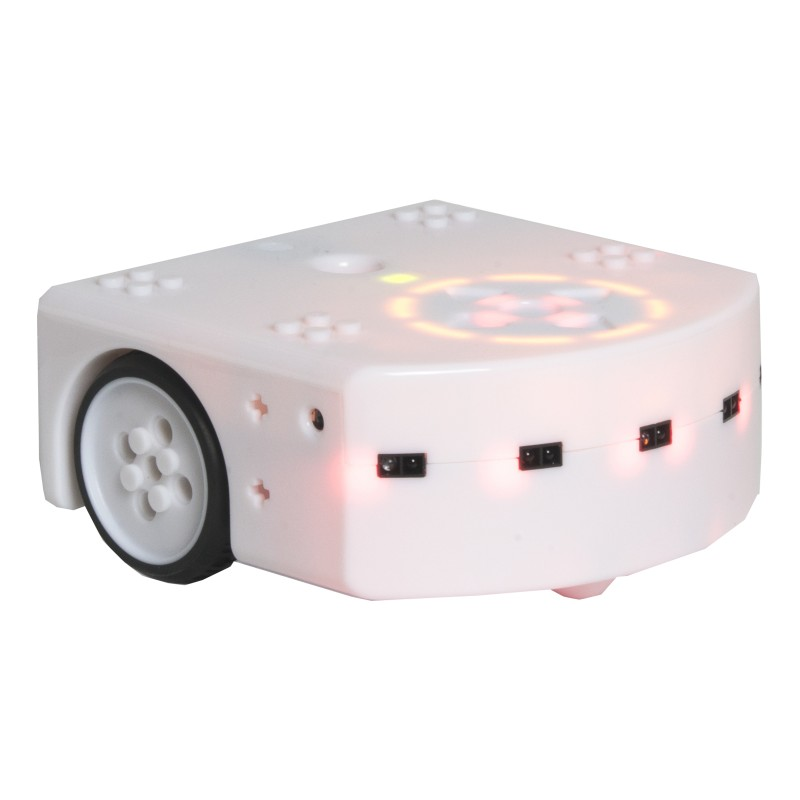
\includegraphics[width=5cm]{ressources/robot-thymio.jpg}
\captionof{figure}{Robot Thymio}
\label{thymio}
\end{center}
Certains comportements ont déjà été programmés dans le robot. Chaque couleur correspond à un programme.
\begin{activite}
\begin{enumerate}
    \item Repérer et compter les capteurs sur le robot.
    \item Quels sont les actionneurs?
    \item Allumer le robot en appuyant 3 secondes sur le bouton central.
    \item Appuyer sur n'importe quelle flèche pour changer de couleur. Il y a six couleurs correspondant chacune à un comportement. Une fois la couleur choisie, un appui bref sur le bouton central lance le programme. Un autre appui bref stoppe l'exécution.
    \item Décrire le comportement du robot pour chaque couleur. Certaines couleurs (bleu et cyan) sont difficiles à comprendre dès maintenant. Il faut se concentrer sur les autres.
    \item Pour éteindre le robot, le prendre dans la main et appuyer longuement sur le bouton central.
\end{enumerate}
\end{activite}
\section{Programmer le robot Thymio}
Un langage, proche de \emph{scratch}, permet de communiquer avec Thymio. Une fois un programme réalisé, il faut le transmettre au robot. La clé USB est un émetteur lié au robot.
\begin{activite} \textbf{Associer le robot à l'ordinateur}
\begin{enumerate}    
    \item Allumer le robot.
    \item Brancher la clé USB à l'ordinateur.
    \item Depuis le bureau, ouvrir le dossier NSI/thymio (ou ISN/thymio).
    \item Démarrer \emph{thymio web bridge blockly et scracth web}. Le robot devrait être repéré.
    \item Démarrer le logiciel \emph{thymio blockly}. Par défaut il s'ouvre avec le navigateur Internet Explorer. Ce logiciel est obsolète.
    \item Copier le lien dans barre adresse de Internet Explorer.
    \item Ouvrir Firefox et coller le lien dans la barre d'adresse.
\end{enumerate}
\end{activite}
\begin{aretenir}[Remarque]
Il est possible que le fait de brancher plusieurs robots en même temps dans la salle, crée des perturbations. Il faudra alors remplacer la clé USB par un câble USB.
\end{aretenir}
Le langage \emph{Blockly} permet de réaliser une \textbf{programmation événementielle:} le robot agit en fonction d'événements extérieurs. De plus il peut réagir à plusieurs événements simultanément. On parle alors de \textbf{programmation parallèle}.
\begin{activite}\textbf{Programmer le robot}
\begin{enumerate}
    \item Créer une instruction qui demande au robot de commencer à avancer quand on appuie sur la flèche avant.
    \item Appuyer sur le bouton d'exécution (figure \ref{execution}). Le bouton \emph{stop} arrête immédiatement l'exécution du programme.
\begin{center}
\centering

\includegraphics[width=2cm]{ressources/execution.png}
\captionof{figure}{Exécuter le programme}
\label{execution}
\end{center}
    \item Ajouter un second événement: le robot doit s'arrêter quand le capteur avant détecte quelque chose. De plus la LED rouge doit s'allumer.
    \item Compléter le programme pour que le robot:
    \begin{itemize}
        \item tourne dans la direction de la flèche pressée,
        \item s'arrête quand on appuie sur le bouton central.
    \end{itemize}
\end{enumerate}
\end{activite}
\end{document}